% Propósito: diferenciar armónicos, parciales, sobretonos, componente de mayor
% amplitud y fundamental ausente mediante espectros con una misma escala.
% Origen: datos teóricos de magnitud normalizada. Panel armónico:
% f=(100,200,300,400) Hz y A=(0,45;1;0,60;0,30). Panel inarmónico:
% f=(100,235,370,520) Hz y A=(0,60;1;0,55;0,30). Fundamental ausente:
% f=(200,300,400) Hz y A=(1;0,60;0,40), con separación de 100 Hz.
% No representa sonidos medidos ni instrumentos particulares.
% Descripción accesible: el primer panel tiene líneas en múltiplos de 100 Hz y
% muestra que el segundo armónico puede superar a la fundamental. El segundo
% presenta parciales que no son múltiplos enteros. El tercero omite la línea de
% 100 Hz, pero conserva líneas separadas 100 Hz, de modo que la periodicidad
% fundamental puede inferirse aunque esa componente esté ausente.
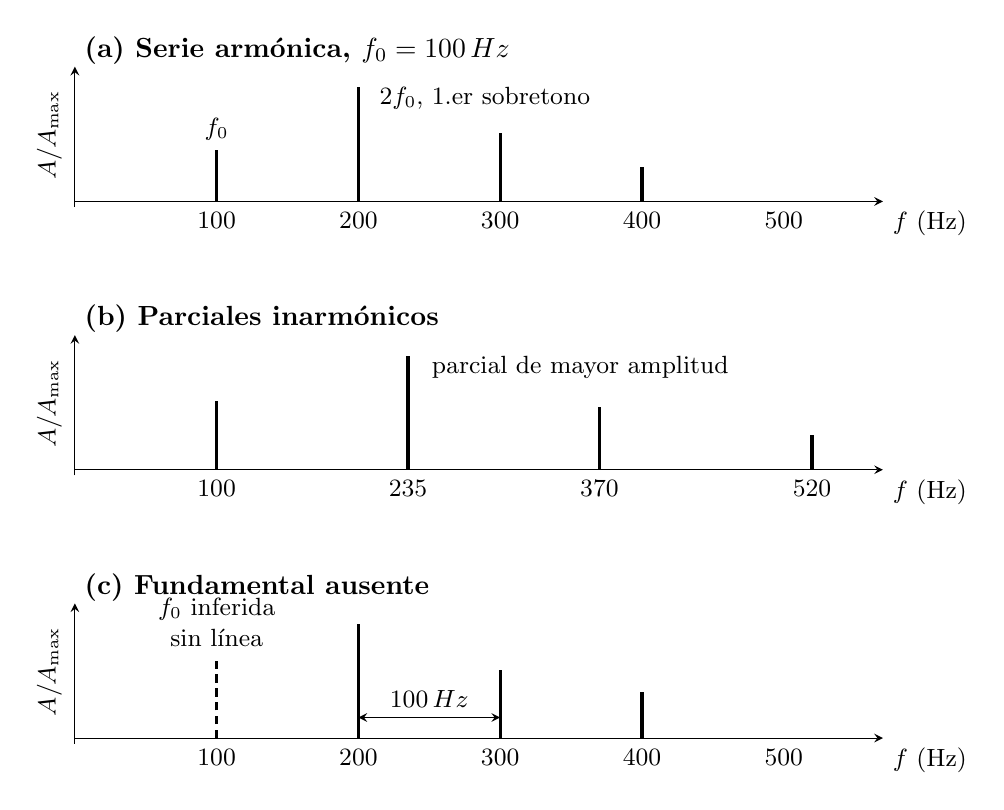
\begin{tikzpicture}[font=\small,>=stealth,x=0.018cm,y=1.45cm]
    \begin{scope}[shift={(0,4.55)}]
        \node[anchor=west,font=\bfseries] at (0,1.32)
            {(a) Serie armónica, \(f_0=100\,\text{Hz}\)};
        \draw[->] (0,0) -- (570,0) node[below right] {\(f\) (Hz)};
        \draw[->] (0,-0.05) -- (0,1.18);
        \node[rotate=90] at (-18,0.58) {\(A/A_{\max}\)};
        \foreach \f/\a in {100/0.45,200/1.00,300/0.60,400/0.30}
            \draw[very thick] (\f,0) -- (\f,\a);
        \foreach \f in {100,200,300,400,500}
            \node[below] at (\f,-0.01) {\f};
        \node[above,align=center] at (100,0.45) {\(f_0\)};
        \node[anchor=west,align=left] at (208,0.90)
            {\(2f_0\), 1.er sobretono};
    \end{scope}

    \begin{scope}[shift={(0,2.20)}]
        \node[anchor=west,font=\bfseries] at (0,1.32)
            {(b) Parciales inarmónicos};
        \draw[->] (0,0) -- (570,0) node[below right] {\(f\) (Hz)};
        \draw[->] (0,-0.05) -- (0,1.18);
        \node[rotate=90] at (-18,0.58) {\(A/A_{\max}\)};
        \foreach \f/\a in {100/0.60,235/1.00,370/0.55,520/0.30}
            \draw[very thick] (\f,0) -- (\f,\a);
        \foreach \f in {100,235,370,520}
            \node[below] at (\f,-0.01) {\f};
        \node[anchor=west] at (245,0.90) {parcial de mayor amplitud};
    \end{scope}

    \begin{scope}[shift={(0,-0.15)}]
        \node[anchor=west,font=\bfseries] at (0,1.32)
            {(c) Fundamental ausente};
        \draw[->] (0,0) -- (570,0) node[below right] {\(f\) (Hz)};
        \draw[->] (0,-0.05) -- (0,1.18);
        \node[rotate=90] at (-18,0.58) {\(A/A_{\max}\)};
        \draw[very thick,densely dashed] (100,0) -- (100,0.72);
        \foreach \f/\a in {200/1.00,300/0.60,400/0.40}
            \draw[very thick] (\f,0) -- (\f,\a);
        \foreach \f in {100,200,300,400,500}
            \node[below] at (\f,-0.01) {\f};
        \node[above,align=center] at (100,0.72)
            {\(f_0\) inferida\\sin línea};
        \draw[<->] (200,0.18) -- (300,0.18)
            node[midway,above] {\(100\,\text{Hz}\)};
    \end{scope}
\end{tikzpicture}
